% section 2: Components

\section{Components}

As in DC2, processing flow in DC3a is guided by three production pipelines. Each of
these pipelines, consisting of a consecutive series of independent stages
linked together via a software harness, will be explained in greater detail below. 
Figure \ref{fig:dc3apipes} diagrams major components of the processing flow in DC3a;
figure \ref{fig:lsstpipes} shows for comparison the baseline design for processing 
flow in the fully implemented LSST.

\begin{itemize}

\item The \textit{image processing and source detection} (IPSD) pipeline takes 
as input the raw exposure images along with the related calibration data and 
produces a catalog of the light sources found within those images. DC3a added
image signature removal to this pipeline, along with the paradigm in which
images are processed in pairs to allow for cosmic ray detection.

\item The \textit{Night Moving Object Processing System} pipeline (NightMOPS) takes
time and coordinate information from the exposure and creates
a catalog of known solar system objects expected to be within
the exposure FOV. It operates in parallel with the IPSD pipeline.

\item The \textit{association pipeline} (AP) then correlates the sources found
by the IPSD with known objects --- either fixed objects or objects expected
by NightMOPS to be within the FOV --- to determine whether new sources
have been detected.

\begin{figure}[t]
\begin{center}
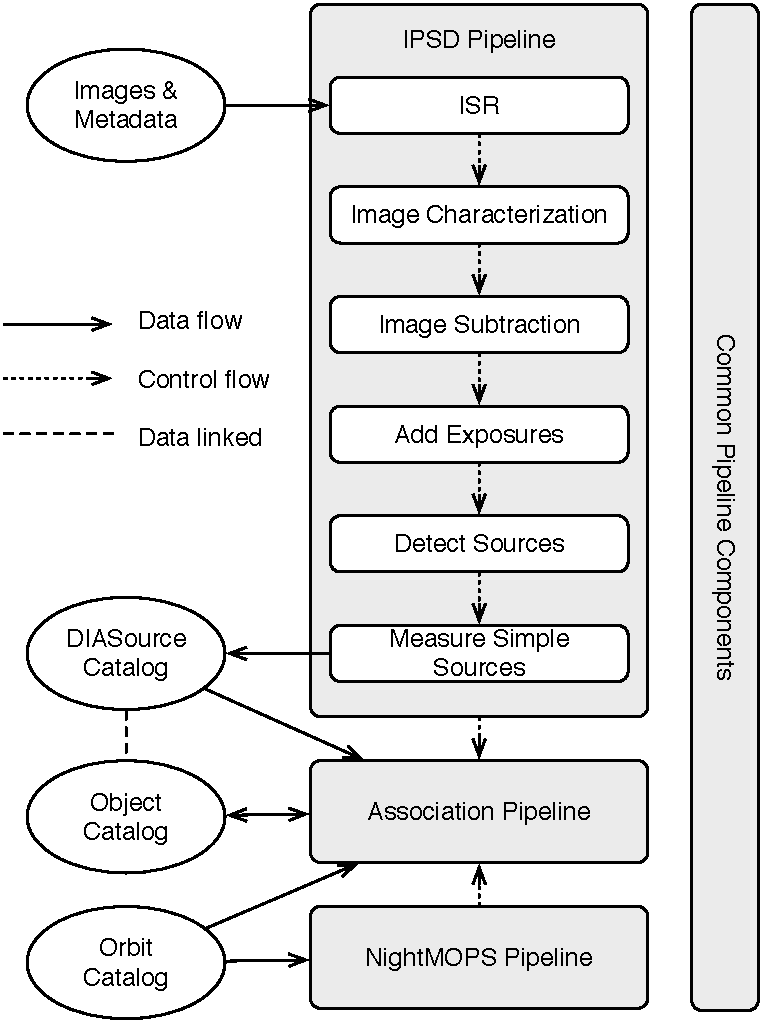
\includegraphics[width=3in]{images/DC3aNightly.pdf}
\caption{Processing flow in DC3a. Three pipelines (IPSD, Association, and
NightMOPS) are supported by a common infrastructure.  
\label{fig:dc3apipes}}
\end{center}
\end{figure}

\begin{figure}[t]
\begin{center}
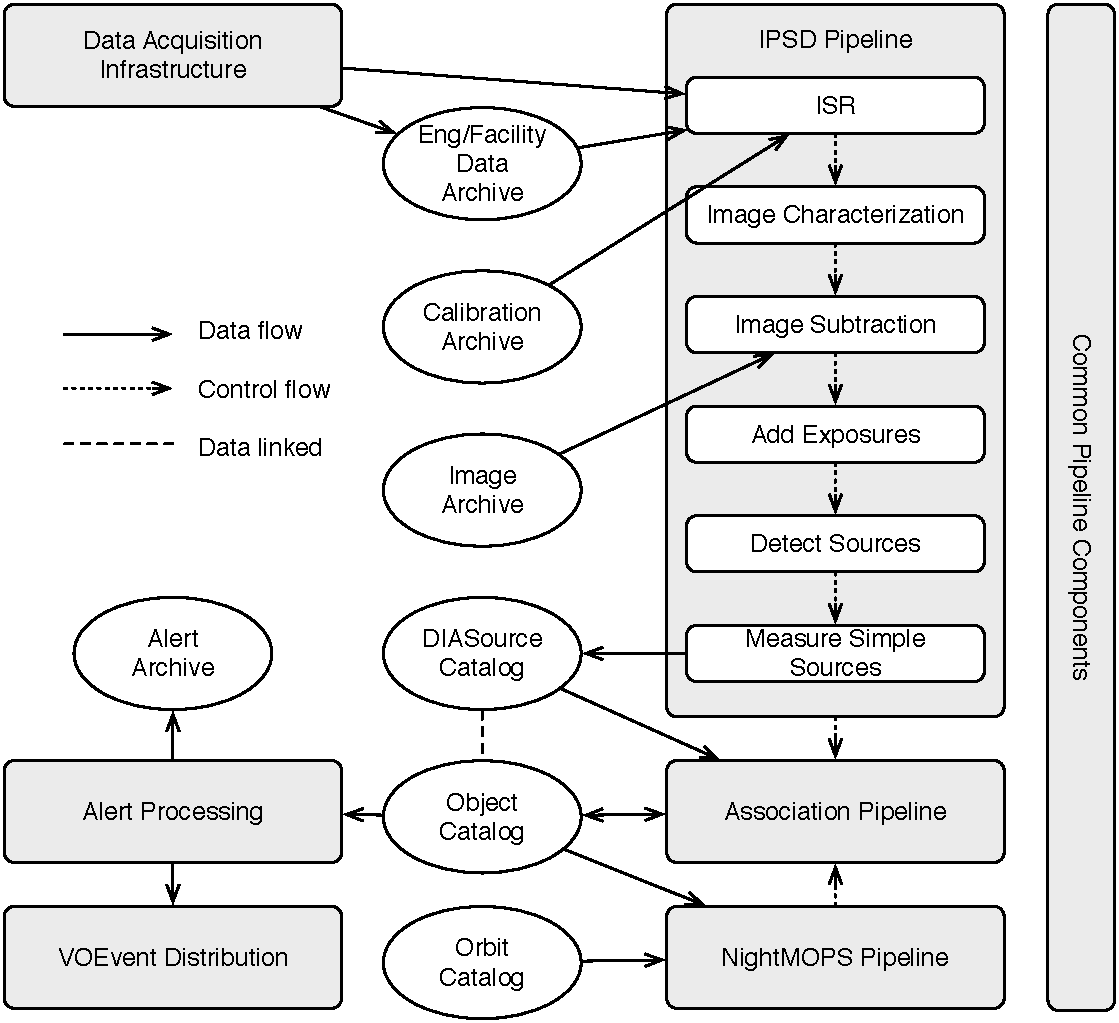
\includegraphics[width=4.5in]{images/LSSTpipes.pdf}
\caption{Baseline design for nightly image processing flow for LSST; DC3a represents
a subset of this design.  
\label{fig:lsstpipes}}
\end{center}
\end{figure}


\end{itemize}

The three pipelines are loosely coupled via event-based communication. 
The whole system is configured via a set of 
human-readable \textit{policy files} which define the different stages which make 
up the pipeline and provide values for parameters that control the behavior of components.
Each pipeline and each application stage within the pipeline has an associated
policy file. 

The pipeline stages are coordinated through an \textit{orchestration layer},
a set of Python objects used to set up and launch pipelines (Section 
\ref{sec:PipelineOrchestration}, page \pageref{sec:PipelineOrchestration}).
An \textit{event broker} serves as a common communication
point among the pipelines, and allows for the capture of execution
logging information for system debugging and performance analysis. 

A shared MySQL database was used to exchange information between the
pipelines.

\subsection{Overview of Processing Flow}

A processing run is triggered by invoking an orchestration layer 
command line utility named \texttt{Orca} with a run ID and a policy file.
The run ID is a unique identifier assigned to a particular processing run,
and all outputs of a run can be associated with their run ID for debugging
or analysis purposes.

Based on the information contained in the \texttt{Orca} policy file, a
pipeline harness is instantiated for each of the three pipelines. For each
exposure pair to be processed, a signal is sent to the event broker to indicate
the availability of the corresponding raw data, whereupon the pipelines 
begin processing.

\subsubsection{Image Processing and Source Detection (IPSD)}

The IPSD pipeline processes images in pairs: two exposures, designated 0 and 1, 
are considered to have been taken consecutively with the same field of view at 
essentially the same time. This pairing of exposures allows for the detection 
of cosmic rays appearing in one exposure but not the other. 

The IPSD performs the following tasks, in sequence:

\begin{itemize}

\item Information is read in identifying the exposures to be processed, and 
links are created in the file system from the working directory to the input
images.

\item For image 0 of the pair, metadata in the FITS file header is read in, 
giving the exposure time, location of the field of view, and similar information, 
which is then persisted to the clipboard.

\item Given this information, the calibration products associated with that
exposure are identified by lookup. Calibration products include darks,
flats, bias, and scatter exposures associated with a given camera run.

\item These calibration products are then used to perform instrument
signature removal (ISR) on the raw exposure, resulting in a calibrated image.

\item Source detection is then performed on calibrated image, giving source
information needed later for determining the WCS coordinates of the
exposure.

\item The point spread function (PSF) of the exposure is determined.

\item The second image of the pair is read in and also goes through ISR.

\item WCS of the exposures is determined.

\item The calibrated exposures are then persisted.

\item A template image representing the ideal expected exposure is
created. When processing CHFT-LS images, these templates are 
resampled from stacked images provided by the CHFT-LS survey.

\item Calibrated images 0 and 1 are subtracted from the template
image, and the difference images created are persisted.

\item These difference images are added together. Source detection
and measurement is then performed. The sources detected are
persisted in the DIASource database.

\item The association pipeline is signaled through the events broker
that the processing of the image pair is complete and that the source
data is ready for the association process.

\item SDQA data from the exposure is persisted.

\end{itemize}

\subsubsection{Night Moving Object Processing System (MOPS)}

The MOPS pipeline performs the following tasks, in sequence:

\begin{itemize}

\item Given the required field of view, MOPS predicts the positions 
of known moving objects in the field.

\item These positions are recorded into the database.

\item MOPS then signals the association pipeline, through the events
broker, that its predictions are available.

\end{itemize}

\subsubsection{Association Pipeline (AP)}

The association pipeline performs the following tasks, in sequence:

\begin{itemize}

\item The pipeline awaits signals from the event broker that
both the IPSD and MOPS pipelines have completed their computations
on a given pair of exposures.

\item New source detections from the DIASource catalog are loaded 
into memory.

\item These detections are matched against known, fixed objects.
Matches are recorded into the database.

\item The MOPS predictions for known moving objects are loaded 
into memory, and the new source detections are matched against
these predictions. Again, matches are recorded in the database.

\item New sources are then used to update the catalog of known
objects.

\end{itemize}

\subsection{Hardware Deployment}

\subsubsection{The NCSA LSST Cluster}

Most of the DC3a preliminary and production runs were performed on a dedicated 
ten-nodes Dell Server Xeon cluster hosted at NCSA. This heterogenous cluster 
consists of two Xeon 3.6 GHz single dual-core nodes, two Xeon 3.6 Ghz dual
dual-core nodes, and six Xeon 2.0 Ghz dual quad-core nodes. It uses a
gigabit ethernet interface.

This cluster was built for DC2 and the DC2 runs were performed there; for DC3, 
the cluster was upgraded from 32-bit Red Hat Enterprise Linux 4 to 64-bit
Red Hat Enterprise Linux 5. Each cluster node has 4 GB memory, with the exception
of \texttt{lsst10}, which has 16 GB. Each node has from 20 to 60 GB of local disk,
along with 15 TB of disk storage shared among nodes using the NFS shared file system.
As part of DC3a, we installed the Lustre parallel file system to increase I/O 
throughput. We were not, however, able to stabilize the Lustre installation
sufficiently to use it for production runs on the NCSA cluster, as planned.

\subsubsection{NCSA Abe}

For purposes of testing the scalability of the pipelines, additional runs were
performed on a larger cluster, Abe, hosted at NCSA. Abe consists of 1200
dual quad-core Xeon 2.33 GHz processors; for the LSST runs we used 36 of these 
nodes, for a total of 288 cores, sufficient to process an entire focal plane 
for the CHFT-LS images. Each core has 1 GB of memory, and shared access
to 100 TB of disk storage as managed using Lustre.

Abe job runs were coordinated using the Condor-G jobs management system.
The events broker and database were not moved to Abe during these runs;
they remained on the LSST cluster.